\begin{frame}
	\frametitle{\secname}

	\begin{theorem}
		If $\theta\in\mathds{R}$, then
		\begin{equation*}
			\operatorname{Re}
			\left(\sum\limits_{k=1}^{n}e^{ik\theta}\right)=
			\sum\limits_{k=1}^{n}
			\operatorname{Re}
			\left(e^{ik\theta}\right)=
			\sum\limits_{k=1}^{n}
			\cos\left(k\theta\right)=
			\begin{cases}
				\dfrac{
					\sin\left(\left(2n+1\right)\frac{\theta}{2}\right)
				}{
					2\sin\left(\frac{\theta}{2}\right)
				}-\dfrac{1}{2},
				 & \exists m\in\mathds{Z}
				\text{ such that }\theta\neq 2m\pi. \\
				n,
				 & \text{otherwise}.
			\end{cases}
		\end{equation*}
	\end{theorem}

	\begin{proof}
		From the geometric sum of $\alert{e^{i\theta}}$ and
		\begin{math}
			2i\sin\left(\theta\right)=
			e^{i\theta}-e^{-i\theta}
		\end{math}:

		\begin{equation*}
			\sum\limits_{k=1}^{n}
			{\left(\alert{e^{i\theta}}\right)}^{k}=
			\frac{
				{\left(\alert{e^{i\theta}}\right)}^{\left(n+1\right)}-
				\alert{e^{i\theta}}
			}{
				\alert{e^{i\theta}}-1
			}=
			e^{i\theta}
			\frac{e^{in\theta}-1}{e^{i\theta}-1}=
			e^{i\theta}
			\frac{
				e^{in\frac{\theta}{2}}
				\left(
				\alert{e^{in\frac{\theta}{2}}-e^{-in\frac{\theta}{2}}}
				\right)
			}{
				e^{i\frac{\theta}{2}}
				\left(
				\alert{e^{i\frac{\theta}{2}}-e^{-i\frac{\theta}{2}}}
				\right)
			}=
			e^{i\left(n+1\right)\frac{\theta}{2}}
			\frac{
				\alert{2i\sin\left(n\frac{\theta}{2}\right)}
			}{
				\alert{2i\sin\left(\frac{\theta}{2}\right)}
			}=
			e^{i\left(n+1\right)\frac{\theta}{2}}
			\frac{
				\sin\left(n\frac{\theta}{2}\right)
			}{
				\sin\left(\frac{\theta}{2}\right)
			}.
		\end{equation*}

		Taking the \alert{real part} on the opposite sides of the
		equality and
		\begin{math}
			\cos\left(\theta_{1}\right)
			\sin\left(\theta_{2}\right)
			=
			\frac{1}{2}
			\left(
			\sin\left(\theta_{1}+\theta_{2}\right)-
			\sin\left(\theta_{1}-\theta_{2}\right)
			\right)
		\end{math}:

		\begin{equation*}
			\cos\left(\alert{\left(n+1\right)\frac{\theta}{2}}\right)
			\frac{
				\sin\left(\alert{n\frac{\theta}{2}}\right)
			}{
				\sin\left(\frac{\theta}{2}\right)
			}=
			\frac{
				\sin\left(
				\alert{\left(n+1\right)\frac{\theta}{2}+n\frac{\theta}{2}}
				\right)-
				\sin\left(
				\alert{\left(n+1\right)\frac{\theta}{2}-n\frac{\theta}{2}}
				\right)
			}{
				\alert{2}\sin\left(\frac{\theta}{2}\right)
			}=
			\frac{
				\sin\left(
				\left(2n+1\right)\frac{\theta}{2}
				\right)-
				\sin\left(\frac{\theta}{2}\right)}{
				2\sin\left(\frac{\theta}{2}\right)
			}.
		\end{equation*}
	\end{proof}
\end{frame}

\begin{frame}
	\frametitle{\secname}

	% Página 238, 386
	\begin{columns}
		\begin{column}{0.42\textwidth}
			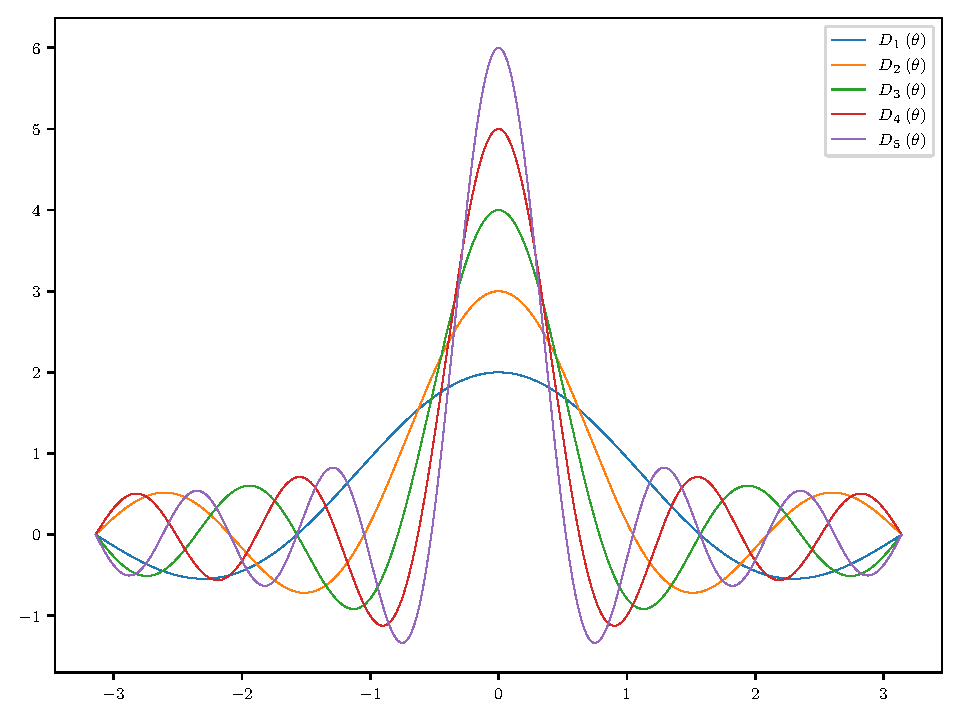
\includegraphics[width=0.35\paperwidth]{plot_dirichlet}
		\end{column}
		\begin{column}{0.54\textwidth}
			\begin{definition}[Dirichlet kernel]
				The \alert{Dirichlet kernel} $D_{n}$ of $n$-order is
				\begin{equation*}
					\fcolorbox{DarkBlue}{yellow}{
						\begin{math}
							\displaystyle
							D_{n}\left(\theta\right)\coloneqq
							\frac{1}{2}+
							\sum\limits_{k=1}^{n}\cos\left(k\theta\right)
						\end{math}
					}
				\end{equation*}
				$2\pi$-periodic and even, i.e.
				\begin{math}
					\forall\theta\in\mathds{R}:
					D\left(-\theta\right)=D\left(\theta\right)
				\end{math}.
			\end{definition}
		\end{column}
	\end{columns}

	\begin{definition}[Periodic function~\cite{Eisermann2023}]
		A function $f\colon\mathds{R}\to\mathds{C}$ is
		$T$-\alert{periodic} iff
		\begin{math}
			\exists T\in\mathds{R}\setminus\left\{0\right\}
		\end{math}
		such that
		\begin{math}
			\forall x\in\mathds{R}:
			f\left(x+T\right)=
			f\left(x\right)
		\end{math}.
	\end{definition}
	% https://math.stackexchange.com/a/3267091 % y par en $\left[0,T\right]$
	% \begin{theorem}[Integral $T$-periodic functions]% 1319p
	% 	The function $f\colon\mathds{R}\to\mathds{C}$ is
	% \end{theorem}
	\begin{block}{Remark}
		Let $x\in\mathds{R}$.
		If $f\in L\left(\left[0,T\right]\right)$ is $T$-periodic,
		then with the change of variable
		\begin{math}
			\alert{
				y\leftarrow\theta+x-\frac{T}{2}
			}
		\end{math}:

		\begin{equation*}
			\int\limits_{0}^{T}f\left(\theta\right)\dl\theta=
			\int\limits_{0}^{\frac{T}{2}}f\left(\theta\right)\dl\theta+
			\int\limits_{\frac{T}{2}}^{T}f\left(\theta\right)\dl\theta=
			\int\limits_{\alert{x-\frac{T}{2}}}^{\alert{x}}f\left(y\right)\dl y+
			\int\limits_{\alert{x}}^{\alert{x+\frac{T}{2}}}f\left(y\right)\dl y=
			\int\limits_{x-\frac{T}{2}}^{x+\frac{T}{2}}f\left(y\right)\dl y.
		\end{equation*}
	\end{block}
\end{frame}

\begin{frame}[allowframebreaks]
	%\frametitle{\secname}
	\begin{lemma}
		If $f\in L\left(\left[0,2\pi\right]\right)$ is $2\pi$-periodic,
		then the sequence of partial sum
		$\left\{s_{n}f\left(\theta\right)\right\}_{n\in\mathds{N}}$ of
		trigonometric Fourier series generated by $f$ has the integral
		representation
		\begin{equation*}
			\fcolorbox{DarkBlue}{yellow}{
				\begin{math}
					\displaystyle
					s_{n}f\left(\theta\right)=
					\frac{2}{\pi}\int\limits_{0}^{\pi}
					\frac{f\left(\theta+\xi\right)+f\left(\theta-\xi\right)}{2}
					D_{n}\left(\xi\right)\dl\xi.
				\end{math}
			}
		\end{equation*}
	\end{lemma}

	\begin{proof}
		\begin{align*}
			s_{n}f\left(\theta\right) & =
			\frac{\alert{a_{0}}}{2}+
			\sum_{k=1}^{n}
			\left(
			\alert{a_{k}}\cos\left(k\theta\right)+
			\alert{b_{k}}\sin\left(k\theta\right)
			\right).                      \\
			s_{n}f\left(\theta\right) & =
			\frac{1}{2}\cdot
			\alert{
				\frac{1}{\pi}
				\int\limits_{0}^{2\pi}
				f\left(\xi\right){\dl\xi}
			}+
			\sum_{k=1}^{n}
			\left(
			\alert{
				\frac{1}{\pi}
				\int\limits_{0}^{2\pi}
				f\left(\xi\right)\cos\left(k\xi\right){\dl\xi}
			}
			\cos\left(k\theta\right)+
			\alert{
				\frac{1}{\pi}
				\int\limits_{0}^{2\pi}
				f\left(\xi\right)\sin\left(k\xi\right){\dl\xi}
			}
			\sin\left(k\theta\right)
			\right).                      \\
			s_{n}f\left(\theta\right) & =
			\alert{
				\frac{1}{\pi}
				\int\limits_{0}^{2\pi}
				f\left(\xi\right)
			}
			\left(
			\frac{1}{2}
			+
			\sum_{k=1}^{n}
			\alert{\cos\left(k\xi\right)}
			\cos\left(k\theta\right)+
			\alert{\sin\left(k\xi\right)}
			\sin\left(k\theta\right)
			\right)
			\alert{{\dl\xi}}=
			\frac{1}{\pi}
			\int\limits_{0}^{2\pi}
			f\left(\xi\right)
			\left(
			\alert{
				\frac{1}{2}
				+
				\sum_{k=1}^{n}
				\cos\left(k\xi-k\theta\right)
			}
			\right)\dl\xi.
		\end{align*}

		\framebreak

		\begin{align*}
			s_{n}f\left(\theta\right) & =
			\frac{1}{\pi}
			\int\limits_{0}^{2\pi}
			f\left(\xi\right)
			\alert{
				D_{n}
				\left(
				k\left(\xi-\theta\right)
				\right)
			}
			\dl\xi.
			\shortintertext{
				The period of the product of two periodic functions $f$ and
				$D_{n}$ is the least common multiple of its periods, i.e.
				$\operatorname{lcm}\left(2\pi,2\pi\right)=2\pi$ and
				plugging the $u$-substitution $\alert{u=\xi-\theta}$.
			}
			s_{n}f\left(\theta\right) & =
			\frac{1}{\pi}
			\int\limits_{\theta-\pi}^{\theta+\pi}
			f\left(\alert{\xi}\right)
			D_{n}
			\left(
			k\left(\alert{\xi-\theta}\right)
			\right)
			\dl\xi=
			\frac{1}{\pi}
			\int\limits_{-\pi}^{\pi}
			f\left(\alert{\theta+u}\right)
			D_{n}
			\left(
			\alert{u}
			\right)
			\dl u.                        \\
			s_{n}f\left(\theta\right) & =
			\frac{1}{\pi}\left(
			\alert{\int\limits_{-\pi}^{0}}
			f\left(\theta+u\right)
			D_{n}
			\left(
			u
			\right)
			\dl u+
			\alert{\int\limits_{0}^{\pi}}
			f\left(\theta+u\right)
			D_{n}
			\left(
			u
			\right)
			\dl u
			\right).                      \\
			s_{n}f\left(\theta\right) & =
			\frac{1}{\pi}\left(
			\int\limits_{-\pi}^{0}
			f\left(\theta+u\right)
			\left(\alert{
				D_{n}
				\left(
				-u
				\right)
			}
			\right)
			\dl u+
			\int\limits_{0}^{\pi}
			f\left(\theta+u\right)
			D_{n}
			\left(
			u
			\right)
			\dl u
			\right).                      \\
			s_{n}f\left(\theta\right) & =
			\frac{1}{\pi}\left(
			\alert{\int\limits_{0}^{\pi}}
			f\left(\theta-u\right)
			D_{n}
			\left(
			u
			\right)
			\dl u+
			\alert{\int\limits_{0}^{\pi}}
			f\left(\theta+u\right)
			D_{n}
			\left(
			u
			\right)
			\dl u
			\right)=
			\frac{\alert{2}}{\pi}
			\alert{\int\limits_{0}^{\pi}}
			\frac{
				f\left(\theta+u\right)+
				f\left(\theta-u\right)
			}{\alert{2}}
			D_{n}
			\left(
			u
			\right)
			\dl u.
		\end{align*}
	\end{proof}
\end{frame}